\documentclass[11pt]{article}
\newcommand{\ArticleShortTitle}{Адаптивный бюджет BVC}
\newcommand{\ArticlePDFTitle}{Адаптивное распределение вычислительного бюджета в многоролевом анализе программных задач}
\usepackage[a4paper,top=22mm,bottom=22mm,left=22mm,right=22mm,headheight=22pt]{geometry}
\usepackage{fontspec}
\defaultfontfeatures{Ligatures=TeX,Scale=MatchLowercase}
\setmainfont{times.ttf}[
  Path=C:/Windows/Fonts/,
  BoldFont=timesbd.ttf,
  ItalicFont=timesi.ttf,
  BoldItalicFont=timesbi.ttf
]
\setsansfont{arial.ttf}[
  Path=C:/Windows/Fonts/,
  BoldFont=arialbd.ttf,
  ItalicFont=ariali.ttf,
  BoldItalicFont=arialbi.ttf
]
\setmonofont{consola.ttf}[
  Path=C:/Windows/Fonts/,
  BoldFont=consolab.ttf,
  ItalicFont=consolai.ttf,
  BoldItalicFont=consolaz.ttf,
  Scale=0.82
]
\usepackage[main=russian,english]{babel}
\usepackage{microtype}

\usepackage{amsmath,amssymb,mathtools}
\usepackage{booktabs,tabularx,array,longtable,multirow}
\usepackage{graphicx}
\graphicspath{{figures/}}
\usepackage{float}
\usepackage[section]{placeins}
\usepackage{caption}
\usepackage{subcaption}
\usepackage{enumitem}
\usepackage{siunitx}
\sisetup{
  output-decimal-marker={,},
  group-separator={\,},
  group-minimum-digits=4,
  detect-all
}
\usepackage{xcolor}
\definecolor{Ink}{HTML}{0F172A}
\definecolor{Muted}{HTML}{475569}
\definecolor{Rule}{HTML}{CBD5E1}
\definecolor{BVC}{HTML}{7C3AED}
\definecolor{Cyan}{HTML}{0EA5E9}
\definecolor{Teal}{HTML}{14B8A6}
\definecolor{Amber}{HTML}{F59E0B}
\definecolor{Soft}{HTML}{F8FAFC}
\usepackage[most]{tcolorbox}
\newtcolorbox{resultbox}[1][]{
  enhanced,
  breakable,
  colback=Soft,
  colframe=BVC,
  boxrule=0.8pt,
  arc=1.5mm,
  left=3mm,right=3mm,top=2mm,bottom=2mm,
  title={#1},
  fonttitle=\bfseries\sffamily,
  coltitle=Ink
}
\newtcolorbox{methodbox}[1][]{
  enhanced,
  breakable,
  colback=white,
  colframe=Rule,
  boxrule=0.6pt,
  arc=1.5mm,
  left=3mm,right=3mm,top=2mm,bottom=2mm,
  title={#1},
  fonttitle=\bfseries\sffamily,
  coltitle=Ink
}

\usepackage{tikz}
\usetikzlibrary{arrows.meta,positioning,shapes.geometric,calc,fit}
\tikzset{
  stage/.style={draw=Rule,rounded corners=2mm,fill=Soft,minimum height=11mm,
    text width=28mm,align=center,font=\small\sffamily},
  gate/.style={diamond,draw=BVC,fill=BVC!7,aspect=1.8,align=center,
    inner sep=1.2mm,font=\small\sffamily},
  flow/.style={-{Latex[length=2.2mm]},thick,draw=Muted},
  note/.style={font=\scriptsize\sffamily,text=Muted,align=center}
}

\usepackage{titlesec}
\titleformat{\section}{\Large\bfseries\sffamily\color{Ink}}{\thesection.}{0.55em}{}
\titleformat{\subsection}{\large\bfseries\sffamily\color{Ink}}{\thesubsection.}{0.55em}{}
\titleformat{\subsubsection}{\normalsize\bfseries\sffamily\color{Ink}}{\thesubsubsection.}{0.55em}{}
\titlespacing*{\section}{0pt}{2.2ex plus .5ex minus .2ex}{1.0ex}
\titlespacing*{\subsection}{0pt}{1.8ex plus .4ex minus .2ex}{0.8ex}

\usepackage{fancyhdr}
\pagestyle{fancy}
\fancyhf{}
\fancyhead[L]{\small\sffamily\color{Muted}\ArticleShortTitle}
\fancyhead[R]{\small\sffamily\color{Muted}Xynapse / BVC}
\fancyfoot[C]{\small\sffamily\color{Muted}\thepage}
\renewcommand{\headrulewidth}{0.4pt}
\renewcommand{\headrule}{\hbox to\headwidth{\color{Rule}\leaders\hrule height \headrulewidth\hfill}}

\usepackage{csquotes}
\usepackage[
  backend=biber,
  style=numeric-comp,
  sorting=nyt,
  maxbibnames=8,
  giveninits=true,
  doi=true,
  url=true,
  isbn=false
]{biblatex}
\addbibresource{references.bib}
\AtBeginBibliography{\footnotesize\sloppy\hbadness=10000\relax}

\usepackage{hyperref}
\hypersetup{
  colorlinks=true,
  linkcolor=BVC,
  citecolor=BVC,
  urlcolor=Cyan,
  pdftitle={\ArticlePDFTitle},
  pdfauthor={Халилов Джабраиль Эльнурович},
  pdfsubject={Экспериментальная оценка BVC},
  pdfkeywords={BVC, SWE-bench Verified, LLM, программирование, Xynapse}
}
\usepackage[nameinlink,noabbrev]{cleveref}

\captionsetup{
  font=small,
  labelfont={bf,sf,color=Ink},
  textfont={color=Muted},
  justification=centering,
  singlelinecheck=false,
  skip=5pt
}
\setlist[itemize]{leftmargin=1.5em,itemsep=0.25em,topsep=0.35em}
\setlist[enumerate]{leftmargin=1.6em,itemsep=0.25em,topsep=0.35em}
\renewcommand{\arraystretch}{1.15}
\setlength{\tabcolsep}{5pt}
\setlength{\parindent}{1.15em}
\setlength{\parskip}{0.18em}
\setlength{\emergencystretch}{4em}
\tolerance=1200

\newcommand{\BVCname}{Bounded Verification Council (BVC)}
\newcommand{\pp}{п.\,п.}
\newcommand{\dataset}{SWE-bench Verified}
\newcommand{\code}[1]{\texttt{#1}}
\newcommand{\sourcehash}[1]{\texttt{\footnotesize #1}}

% Auto-generated by generate_analysis_assets.py. Do not edit by hand.
\newcommand{\NTasks}{60}
\newcommand{\NRepos}{11}
\newcommand{\NPrimaryRuns}{240}
\newcommand{\NRepeatRuns}{90}
\newcommand{\NVibeRuns}{45}
\newcommand{\NAllRuns}{375}
\newcommand{\DirectResolved}{4}
\newcommand{\SingleResolved}{7}
\newcommand{\BVCResolved}{5}
\newcommand{\FixedResolved}{6}
\newcommand{\DirectRate}{6.7}
\newcommand{\SingleRate}{11.7}
\newcommand{\BVCRate}{8.3}
\newcommand{\FixedRate}{10.0}
\newcommand{\DirectWilsonLow}{2.6}
\newcommand{\DirectWilsonHigh}{15.9}
\newcommand{\SingleWilsonLow}{5.8}
\newcommand{\SingleWilsonHigh}{22.2}
\newcommand{\BVCWilsonLow}{3.6}
\newcommand{\BVCWilsonHigh}{18.1}
\newcommand{\FixedWilsonLow}{4.7}
\newcommand{\FixedWilsonHigh}{20.1}
\newcommand{\BVCCalls}{472}
\newcommand{\FixedCalls}{600}
\newcommand{\DirectCalls}{60}
\newcommand{\SingleCalls}{120}
\newcommand{\BVCTokens}{14282809}
\newcommand{\FixedTokens}{18365172}
\newcommand{\DirectTokens}{1867093}
\newcommand{\SingleTokens}{3585838}
\newcommand{\BVCCost}{1838.46}
\newcommand{\FixedCost}{2402.61}
\newcommand{\DirectCost}{312.44}
\newcommand{\SingleCost}{522.84}
\newcommand{\BVCCostTask}{30.64}
\newcommand{\FixedCostTask}{40.04}
\newcommand{\DirectCostTask}{5.21}
\newcommand{\SingleCostTask}{8.71}
\newcommand{\BVCCostResolved}{367.69}
\newcommand{\FixedCostResolved}{400.44}
\newcommand{\DirectCostResolved}{78.11}
\newcommand{\SingleCostResolved}{74.69}
\newcommand{\CallsSaved}{128}
\newcommand{\CallsSavedPct}{21.3}
\newcommand{\TokensSaved}{4082363}
\newcommand{\TokensSavedPct}{22.2}
\newcommand{\CostSaved}{564.15}
\newcommand{\CostSavedPct}{23.5}
\newcommand{\CostResolvedSavedPct}{8.2}
\newcommand{\TokensSavedTask}{68039}
\newcommand{\CostSavedTask}{9.40}
\newcommand{\CallsSavedTaskMean}{2.13}
\newcommand{\CallsSavedTaskMeanLow}{1.60}
\newcommand{\CallsSavedTaskMeanHigh}{2.67}
\newcommand{\CallsSavedTaskMedian}{4}
\newcommand{\TokensSavedTaskMeanLow}{51980}
\newcommand{\TokensSavedTaskMeanHigh}{83480}
\newcommand{\TokensSavedTaskMedian}{111910}
\newcommand{\CostSavedTaskMeanLow}{6.75}
\newcommand{\CostSavedTaskMeanHigh}{12.05}
\newcommand{\CostSavedTaskMedian}{7.92}
\newcommand{\TokensOverrunTasks}{11}
\newcommand{\TokensOverrunMax}{13971}
\newcommand{\CostOverrunTasks}{10}
\newcommand{\CostOverrunMax}{12.84}
\newcommand{\BVCShort}{32}
\newcommand{\BVCExtended}{28}
\newcommand{\BVCShortResolved}{5}
\newcommand{\BVCExtendedResolved}{0}
\newcommand{\BVCShortTokensMean}{179160}
\newcommand{\BVCExtendedTokensMean}{305345}
\newcommand{\BVCShortCostMean}{22.78}
\newcommand{\BVCExtendedCostMean}{39.62}
\newcommand{\FixedShortResolved}{5}
\newcommand{\FixedExtendedResolved}{1}
\newcommand{\GateUndefinedVote}{7}
\newcommand{\GateFourValidAxes}{35}
\newcommand{\GateThreeValidAxes}{18}
\newcommand{\GateZeroValidAxes}{7}
\newcommand{\GateMetricCorrelation}{0.412}
\newcommand{\AllTokens}{54533372}
\newcommand{\AllCost}{7266.84}
\newcommand{\CostCap}{11800}



\title{\vspace{-1.2em}\textbf{\sffamily Адаптивное распределение вычислительного бюджета\\
в многоролевом анализе программных задач}}
\author{Халилов Джабраиль Эльнурович\\
\small Национальный исследовательский университет «Высшая школа экономики»\\
\small Исследовательский проект Xynapse / BVC\\
\small \href{https://github.com/jabrailkhalil/xynapse}{\nolinkurl{github.com/jabrailkhalil/xynapse}}}
\date{2026}

\begin{document}
\maketitle

\begin{abstract}
Многоролевой анализ программной задачи позволяет до изменения кода независимо
проверить локализацию дефекта, стратегию исправления, затрагиваемые зависимости
и тестовое покрытие. \BVCname{} превращает такую проверку из режима с постоянной
ценой в управляемый сервис: второй раунд критики запускается только после
формализованной проверки расхождения и полноты, а верхняя граница бюджета
известна до старта.
Эксперимент выполнен на \NTasks{} реальных задачах \dataset{} из \NRepos{}
открытых Python-репозиториев. Адаптивный алгоритм обработал \BVCShort{} задачи
за 6 модельных вызовов и направил \BVCExtended{} задач на расширенный
10-вызовный маршрут. Относительно совета с обязательной критикой число вызовов
уменьшилось с \FixedCalls{} до \BVCCalls{} (на \CallsSavedPct\%), объём
токенов --- с \num{\FixedTokens} до \num{\BVCTokens} (на
\TokensSavedPct\%), расчётная стоимость --- с \num{\FixedCost} до
\num{\BVCCost} руб. (на \CostSavedPct\%). BVC решил \BVCResolved{}/\NTasks{}
задач, полный совет --- \FixedResolved{}/\NTasks{}; пять успешных задач
совпали, а одна была решена только полным советом
(разность \(-1{,}7\) \pp, \(p=1{,}0\)). Таким образом, BVC продемонстрировал
практически значимую способность избирательно расходовать inference-time
бюджет и дал прозрачное объяснение каждого решения gate; равенство,
неухудшаемость и превосходство функционального качества не установлены.
\end{abstract}

\noindent\textbf{Ключевые слова:} большие языковые модели, программная
инженерия, многоагентные системы, адаптивная критика, вычислительный бюджет,
\dataset{}, BVC.

\section{Введение}

Современный AI-ассистент способен не только сформировать patch, но и разложить
задачу на несколько независимых инженерных позиций. Архитектор локализует
причину и границы изменения; разработчик предлагает конкретную реализацию;
рецензент проверяет инварианты и совместимость; тестировщик формулирует
наблюдаемое поведение. Многоролевые диалоги и iterative refinement уже
используются как способы увеличить полноту рассуждения
\cite{wu2023autogen,du2023debate,shinn2023reflexion,madaan2023selfrefine}.
Практическая проблема состоит в том, что каждый дополнительный раунд оплачивается
вызовами модели, входным контекстом и выходными токенами.

Архитектура Xynapse IDE и первоначальная модель Bounded Verification Council были
сформулированы в выпускной квалификационной работе автора
\cite{khalilov2026}. Настоящее исследование продолжает дипломную работу
исполняемой проверкой одного конкретного свойства: может ли заранее включаемый
человеком многоролевой анализ тратить полный бюджет избирательно, а не на
каждой задаче. Актуальная программная реализация Xynapse развивается в открытом
репозитории проекта \cite{xynapse2026}; ссылка на репозиторий фиксирует кодовую
реализацию, тогда как диплом остаётся источником архитектуры и постановки метода.

В статье рассматривается не неограниченная дискуссия агентов, а управляемый
процесс с двумя заранее известными маршрутами. После независимого первого
раунда вычисляются две диагностические величины. Если позиции достаточно
полны и согласованы, система сразу синтезирует план; иначе выполняется ровно
один раунд взаимной критики. Поэтому верхняя граница цены известна до запуска,
а фактическая цена определяется наблюдаемым состоянием анализа.

\begin{resultbox}[Вклад работы]
\begin{enumerate}
  \item задана исполняемая функция маршрутизации между 6 и 10 вызовами;
  \item проведено парное сравнение BVC с полным советом на 60 одних и тех же
        задачах и одинаковом кодовом контексте;
  \item экономия разложена по вызовам, токенам, рублям, задачам и успешным
        решениям;
  \item качество patch сохранено как обязательная контрольная метрика:
        все результаты прошли официальный тестовый контур \dataset{}.
\end{enumerate}
\end{resultbox}

\begin{resultbox}[Практическая сила BVC]
Алгоритм объединяет четыре свойства, редко доступные одновременно:
\begin{itemize}
  \item \textbf{предсказуемость:} до запуска известен диапазон 6--10 вызовов;
  \item \textbf{адаптивность:} полный бюджет оплачивается только при
        измеримом расхождении или неполноте первого раунда;
  \item \textbf{объяснимость:} решение gate восстанавливается по
        \(D_{\mathrm{vote}}\), \(D_{\mathrm{cov}}\) и замороженным порогам;
  \item \textbf{измеримость:} экономия получена в end-to-end запуске и
        рассчитана по фактическим вызовам, токенам и тарифным категориям.
\end{itemize}
Тем самым BVC делает многоролевой анализ не дорогой опцией
\enquote{всё или ничего}, а контролируемым уровнем инженерной проверки.
\end{resultbox}

\section{Связанные подходы и постановка задачи}

AutoGen формализует многоагентный разговор как композицию ролей и сообщений
\cite{wu2023autogen}; multiagent debate исследует ценность независимых
позиций и последующего обмена аргументами \cite{du2023debate}. Reflexion и
Self-Refine показывают общий принцип улучшения ответа во время генерации через
обратную связь и повторную переработку
\cite{shinn2023reflexion,madaan2023selfrefine}. Adaptive-Consistency вводит
остановку по наблюдаемому согласию выборок, а FrugalGPT рассматривает
адаптивный каскад моделей как способ управлять ценой
\cite{aggarwal2023adaptive,chen2023frugalgpt}. Во всех этих схемах
дополнительное рассуждение является ресурсом. Инженерная задача состоит не
только в том, чтобы иметь возможность потратить больше вычислений, но и в том,
чтобы определить достаточный момент остановки.

BVC отличается тремя ограничениями. Во-первых, независимые ответы ролей
структурированы по общим осям, поэтому сравниваются решения, а не свободная
формулировка. Во-вторых, второй раунд ограничен единицей. В-третьих, gate
заранее заморожен и не изменяется после просмотра результатов. Исследовательский
вопрос формулируется так:

\begin{quote}
\emph{Насколько адаптивный BVC сокращает фактический расход относительно
полного совета с обязательной критикой и какой функциональный результат
наблюдается при этом сокращении?}
\end{quote}

\section{Алгоритм BVC}

\subsection{Роли и четыре оси решения}

Первый раунд состоит из четырёх независимых вызовов. Каждая роль возвращает
типизированные решения по множеству
\[
\mathcal{A}=
\{\textit{root cause},\textit{fix strategy},
  \textit{dependencies},\textit{test coverage}\}.
\]
Для локализации, поверхности изменения и покрытия используется расстояние
Жаккара между множествами \cite{kosub2019jaccard}; для стратегии --- расстояние между значениями
замороженного категориального словаря. Свободный пояснительный текст в
голосование не входит. Для двух пустых множеств расстояние принято равным нулю;
для пустого и непустого --- единице. Это соглашение совпадает с реализацией,
зафиксированной до основной серии.

Пусть \(V_a\) --- множество валидных решений ролей по оси \(a\), а
\(d_a(i,j)\in[0,1]\) --- расстояние между двумя решениями. При
\(|V_a|\geq2\) среднее попарное расхождение равно
\[
D_a =
\frac{2}{|V_a|(|V_a|-1)}
\sum_{\substack{i<j\\i,j\in V_a}} d_a(i,j).
\]
Общая величина расхождения вычисляется только по осям, на которых доступны
минимум два валидных голоса:
\[
D_{\mathrm{vote}} =
\frac{1}{|\mathcal{A}^{\ast}|}
\sum_{a\in\mathcal{A}^{\ast}} D_a,\qquad
\mathcal{A}^{\ast}=\{a:|V_a|\geq2\}.
\]

Второй показатель отражает не различие ответов, а потерю структуры. Из
\(4\times4=16\) ячеек «роль--ось» подсчитываются отсутствующие или
невалидные:
\[
D_{\mathrm{cov}} =
\frac{N_{\mathrm{missing}}+N_{\mathrm{invalid}}}{16}.
\]
Такое разделение важно: единодушно пропущенная зависимость может иметь низкое
\(D_{\mathrm{vote}}\), но высокое \(D_{\mathrm{cov}}\).

\subsection{Замороженный gate и число вызовов}

Пороговые значения до запуска основной серии были зафиксированы как
\[
\tau_{\mathrm{vote}}=0{,}30,\qquad
\tau_{\mathrm{cov}}=0{,}25.
\]
Это инженерные значения этапа проектирования: они не подбирались по outcomes
60 задач и не заявляются оптимальными. Их назначение --- сделать правило
исполняемым до просмотра результата; post-hoc чувствительность маршрутов к
порогам анализируется отдельно. Поскольку \(D_{\mathrm{vote}}\) не определено
при \(\mathcal{A}^{\ast}=\varnothing\), правило записывается в охраняемой форме:
\[
I_{\mathrm{crit}} =
\begin{cases}
1, & \mathcal{A}^{\ast}=\varnothing,\\[2pt]
\mathbb{1}\!\left[
D_{\mathrm{vote}}>\tau_{\mathrm{vote}}
\;\lor\;
D_{\mathrm{cov}}>\tau_{\mathrm{cov}}
\right], & \mathcal{A}^{\ast}\neq\varnothing.
\end{cases}
\]
Общее число успешных модельных вызовов на задачу:
\[
C_{\mathrm{BVC}}=4+4I_{\mathrm{crit}}+1+1
=6+4I_{\mathrm{crit}}.
\]
Первые четыре слагаемых --- независимые роли; при необходимости ещё четыре
вызова выполняют критику; затем один вызов синтезирует план и один формирует
patch. Полный совет всегда использует
\(C_{\mathrm{fixed}}=10\).

\begin{figure}[H]
\centering
\resizebox{0.98\textwidth}{!}{%
\begin{tikzpicture}[node distance=7mm and 9mm]
  \node[stage] (human) {Человек включает BVC до первой правки};
  \node[stage, right=of human, text width=31mm] (roles) {4 независимые роли\\4 вызова};
  \node[gate, right=of roles] (gate) {\(D_{\mathrm{vote}}\),\\\(D_{\mathrm{cov}}\)};
  \node[stage, above right=4mm and 11mm of gate] (crit) {Взаимная критика\\+4 вызова};
  \node[stage, below right=4mm and 11mm of gate] (synth) {Синтез плана\\1 вызов};
  \node[stage, right=of synth] (patch) {Генерация patch\\1 вызов};
  \draw[flow] (human) -- (roles);
  \draw[flow] (roles) -- (gate);
  \draw[flow] (gate) -- node[note,above left]{порог превышен} (crit);
  \draw[flow] (crit.south) -- (synth.north);
  \draw[flow] (gate) -- node[note,below left]{порог не превышен} (synth);
  \draw[flow] (synth) -- (patch);
\end{tikzpicture}
}
\caption{Два ограниченных маршрута BVC: 6 либо 10 модельных вызовов.}
\label{fig:bvc-flow}
\end{figure}

\subsection{Аналитическая экономия по числу вызовов}

Пусть \(p=\Pr(I_{\mathrm{crit}}=1)\) --- наблюдаемая доля задач с критикой.
Среднее число вызовов тогда равно
\[
\mathbb{E}[C_{\mathrm{BVC}}]=6+4p,
\]
а относительная экономия против полного совета:
\[
S_C = 1-\frac{6+4p}{10}=0{,}4(1-p).
\]
В эксперименте \(p=28/60=0{,}4667\), поэтому
\[
\mathbb{E}[C_{\mathrm{BVC}}]=7{,}8667,\qquad
S_C=0{,}2133.
\]
Это точно соответствует фактическим \(\BVCCalls=32\cdot6+28\cdot10\)
вызовам и экономии \(\CallsSaved=600-472\) вызовов.

\subsection{Расчёт стоимости}

Для каждого запуска сохранялись некэшированные входные токены
\(T_u\), кэшированные входные токены \(T_c\) и выходные токены \(T_o\).
По замороженному тарифу стоимость вычислялась как
\[
R =
0{,}30\frac{T_u}{1000}
+0{,}075\frac{T_c}{1000}
+0{,}50\frac{T_o}{1000}\quad\text{руб.}
\]
Это расчётный тариф, замороженный в протоколе до основной генерации, а не
заявление о фактическом счёте или будущей цене провайдера. Он нужен только для
одинакового сопоставления методов внутри одной экспериментальной матрицы;
пересчёт по другому тарифу не требует повторной генерации.

\section{Экспериментальный дизайн}

\subsection{Задачи и общий контекст}

Использована outcome-blind выборка из \NTasks{} задач \dataset{}
\cite{jimenez2024swebench,openai2024verified}: 30 задач страты medium,
27 --- hard и 3 --- very hard. Из замороженной ревизии на 500 задач были
взяты все три instance трудоёмкостью более четырёх часов, 27 из 42 задач
страты 1--4 часа и 30 из 261 задачи страты 15 минут--1 час; задачи проще
15 минут не включались, поскольку BVC предполагается включать осознанно для
нетривиальной работы. Квоты репозиториев распределялись пропорционально
квадратному корню из размера доступного пула, а внутри квоты порядок
определял SHA-256 от фиксированного seed и \code{instance\_id}. Issue,
эталонный patch и результаты моделей в отборе не участвовали.

Задачи относятся к \NRepos{} репозиториям, включая Django, SymPy, Sphinx,
Astropy, pytest, xarray и scikit-learn. Для всех методов по каждой задаче
передавались одно и то же issue и одни и те же исходные файлы. Использован
замороженный результат BM25 retrieval \cite{robertson2009bm25}: от двух до
восьми файлов, от 71\,369 до 111\,192 символов на задачу, всего 245 файлов
и 5\,691\,570 символов. Из официального retrieval-артефакта извлекались
только блоки исходного кода; демонстрационный patch из legacy-поля
\code{text} в prompt не передавался. Все 245 файлов были независимо сверены
с нужными base commit побайтно.

\subsection{Сравниваемые методы}

Для ответа на вопрос об адаптивном бюджете ресурсно наиболее сопоставимая
пара --- BVC и полный совет. У них совпадают роли, схема решений, синтезатор,
финальная инструкция patch и верхняя граница в 10 вызовов. Единственное
операционное различие состоит в том, что полный совет всегда проводит
критику, а BVC применяет замороженный gate. Дополнительными ориентирами
служат прямой patch одним вызовом и один предварительный план плюс patch
двумя вызовами.

\begin{table}[H]
\centering
\caption{Матрица методов основной серии.}
\label{tab:methods}
\begin{tabularx}{\textwidth}{@{}lXcc@{}}
\toprule
Метод & Предварительный анализ & Вызовы на задачу & Запусков\\
\midrule
Direct & отсутствует & 1 & 60\\
Один план & один структурированный план & 2 & 60\\
BVC & 4 роли; критика по gate; синтез & 6 или 10 & 60\\
Полный совет & 4 роли; обязательная критика; синтез & 10 & 60\\
\bottomrule
\end{tabularx}
\end{table}

Все методы использовали одну версию модели, temperature \(=0\), одинаковые
лимиты финального patch и официальный исполняемый evaluator. Единицей анализа
являлась задача; результаты сопоставлялись попарно. Доля решённых задач
дополнена 95\% Wilson-интервалом \cite{wilson1927}; парные различия ---
точным двусторонним критерием Мак-Немара \cite{mcnemar1947} и
стратифицированным paired bootstrap на 10\,000 выборок
\cite{efron1993bootstrap}.

\subsection{Что именно было запущено}

Конфигурация генерации была общей для всей основной матрицы: Yandex Cloud AI
Studio, запрошенный идентификатор \code{deepseek-v4-flash}, возвращённый URI
\code{gpt://deepseek-v4-flash/latest}, temperature \(=0\), prompt-версия
\code{main60-3.0.0}. Provider seed отсутствовал, поэтому нулевая температура
не трактовалась как гарантия детерминизма. Отдельный параметр
thinking/non-thinking в запросе не передавался: использовался режим по умолчанию
данного URI, а возвращённое поле \code{reasoning\_content} сохранялось
\cite{yandex2026deepseekv4}. Лимит ответа роли и
плана/синтеза составлял 4\,096 токенов, лимит финального unified diff ---
16\,384 токена. Порядок четырёх методов вращался по детерминированному
расписанию \code{bvc-main60-schedule-v1}, чтобы один метод не выполнялся
систематически первым или последним.

Для каждого \code{instance\_id} процедура состояла из шести проверяемых
этапов:
\begin{enumerate}
  \item загрузить только issue, repository, base commit и общий
        context-manifest; difficulty, gold patch, test patch,
        \code{FAIL\_TO\_PASS} и \code{PASS\_TO\_PASS} были закрыты от модели;
  \item выполнить замороженную последовательность вызовов выбранного метода;
  \item сохранить prompt, ответ, usage, finish reason, лимит и SHA-256
        каждого вызова;
  \item извлечь один repository-root unified diff без ручного ремонта;
  \item применить его к чистому checkout нужного base commit;
  \item запустить официальный контейнерный evaluator: успехом считался только
        проход всех обязательных fail-to-pass и pass-to-pass тестов.
\end{enumerate}
Шесть отдельных development-задач использовались для отладки формата и
harness и навсегда исключены из 60-задачной статистики. Пустой,
неразбираемый или неприменимый patch оставался неуспешным outcome, а не
удалялся из данных.

\section{Результаты}

\subsection{Маршрутизация gate}

Короткий маршрут был выбран для \BVCShort{}/60 задач (53,3\%), расширенный
--- для \BVCExtended{}/60 (46,7\%). Следовательно, механизм действительно
адаптировал бюджет: он не выродился ни в постоянные 6, ни в постоянные
10 вызовов.

\begin{figure}[H]
\centering
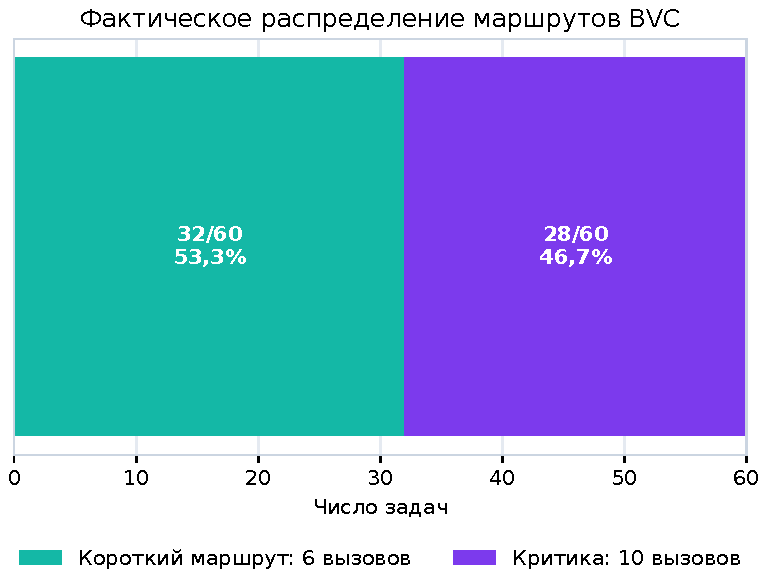
\includegraphics[width=0.82\textwidth]{fig_bvc_routes}
\caption{Фактическая доля двух маршрутов BVC.}
\label{fig:routes}
\end{figure}

Частота критики составила 43,3\% в medium, 48,1\% в hard и 66,7\% в
very hard. Последняя оценка основана только на трёх задачах и потому
показывается как описание выборки, а не как устойчивый тренд.

\begin{figure}[H]
\centering
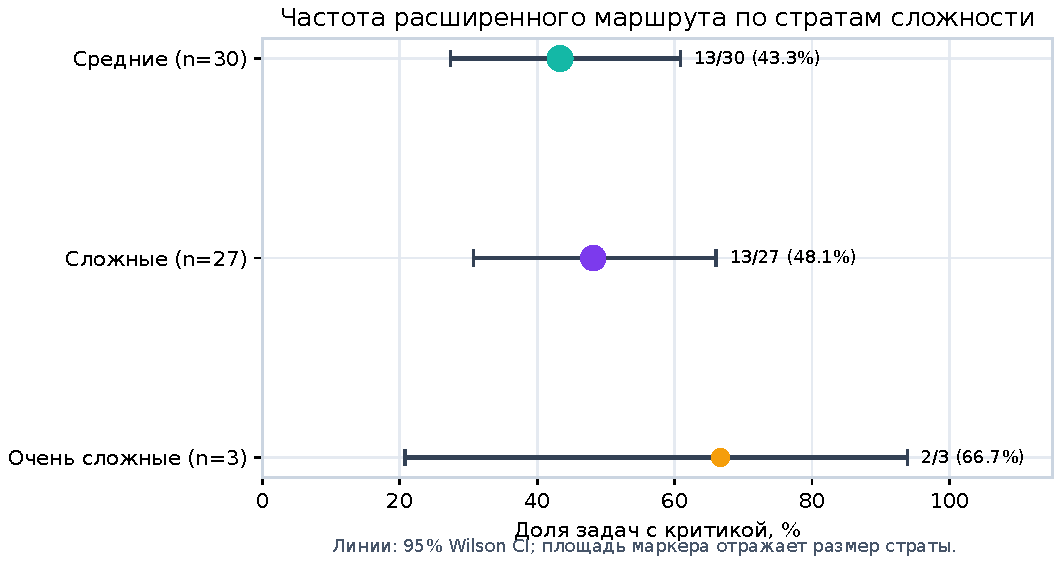
\includegraphics[width=0.75\textwidth]{fig_gate_by_difficulty}
\caption{Частота расширенного маршрута в трёх заранее заданных стратах сложности.}
\label{fig:gate-difficulty}
\end{figure}

На плоскости \((D_{\mathrm{vote}},D_{\mathrm{cov}})\) видна работа двух
числовых порогов. Часть расширенных маршрутов определяется также третьим
условием --- отсутствием оси с двумя валидными голосами. В первом раунде все
четыре оси имели минимум два валидных голоса у \GateFourValidAxes{} задач,
три оси --- у \GateThreeValidAxes{}, ни одной --- у \GateZeroValidAxes{};
других значений не наблюдалось. Для \(\GateUndefinedVote{}\) последних задач
\(D_{\mathrm{vote}}\) не определялось. Среди остальных \(n=53\) задач
корреляция Пирсона между \(D_{\mathrm{vote}}\) и \(D_{\mathrm{cov}}\) равна
\(r=\GateMetricCorrelation\): показатели связаны, но не дублируют друг друга.

\begin{figure}[H]
\centering
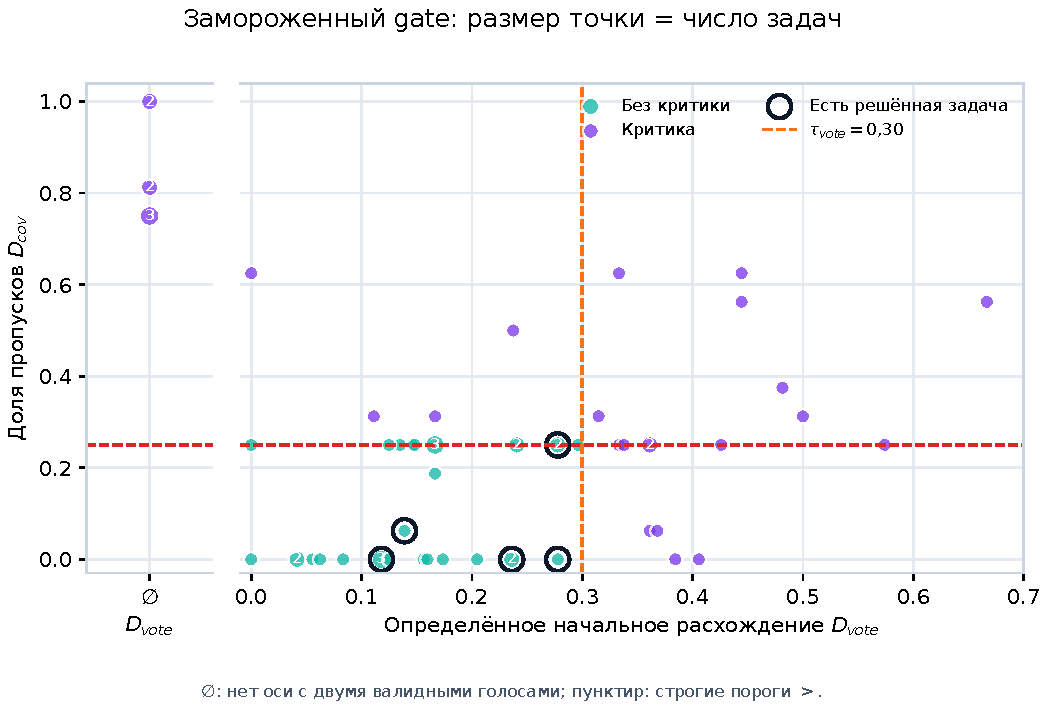
\includegraphics[width=0.88\textwidth]{fig_gate_scatter}
\caption{Начальные диагностические значения, решение gate и функциональный исход.}
\label{fig:gate-scatter}
\end{figure}

Post-hoc анализ порогов изменяет только контрфактическое решение маршрутизации
на уже сохранённых диагностических значениях. Он не пересчитывает планы,
patch или outcomes и потому не является поиском лучшего порога по качеству.

\begin{figure}[H]
\centering
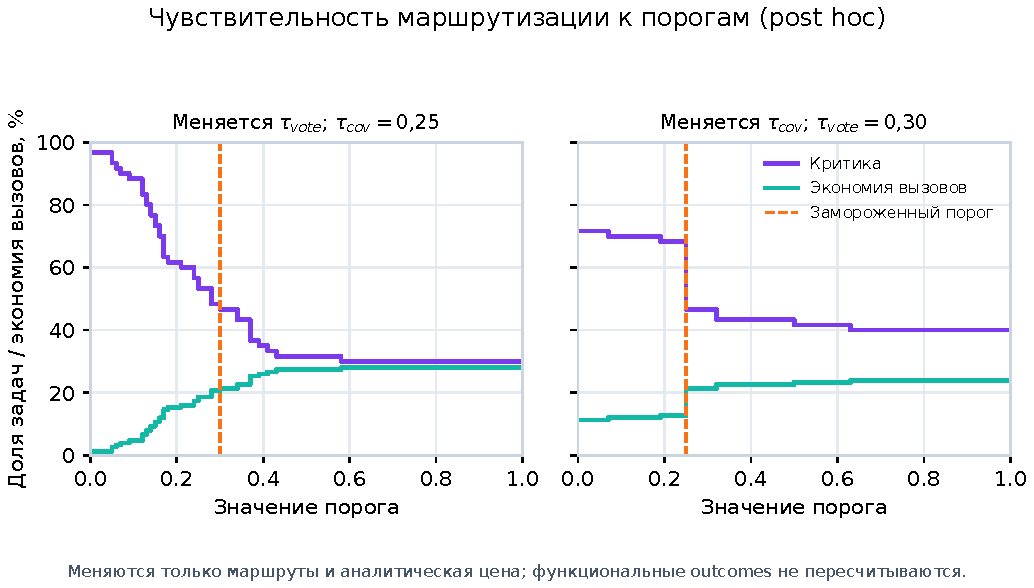
\includegraphics[width=0.94\textwidth]{fig_gate_sensitivity}
\caption{Чувствительность доли критики и аналитической экономии вызовов к
порогам; оранжевым отмечена замороженная конфигурация.}
\label{fig:gate-sensitivity}
\end{figure}

\subsection{Экономия вызовов, токенов и стоимости}

\begin{table}[H]
\centering
\caption{Ресурсный результат BVC относительно полного совета.}
\label{tab:efficiency}
\begin{tabular}{@{}lrrr@{}}
\toprule
Метрика & Полный совет & BVC & Экономия\\
\midrule
Модельные вызовы & \num{\FixedCalls} & \num{\BVCCalls} &
\num{\CallsSaved} (\CallsSavedPct\%)\\
Токены & \num{\FixedTokens} & \num{\BVCTokens} &
\num{\TokensSaved} (\TokensSavedPct\%)\\
Расчётная стоимость, руб. & \num{\FixedCost} & \num{\BVCCost} &
\num{\CostSaved} (\CostSavedPct\%)\\
Стоимость на задачу, руб. & \num{\FixedCostTask} & \num{\BVCCostTask} &
\num{\CostSavedTask}\\
\bottomrule
\end{tabular}
\end{table}

\begin{figure}[H]
\centering
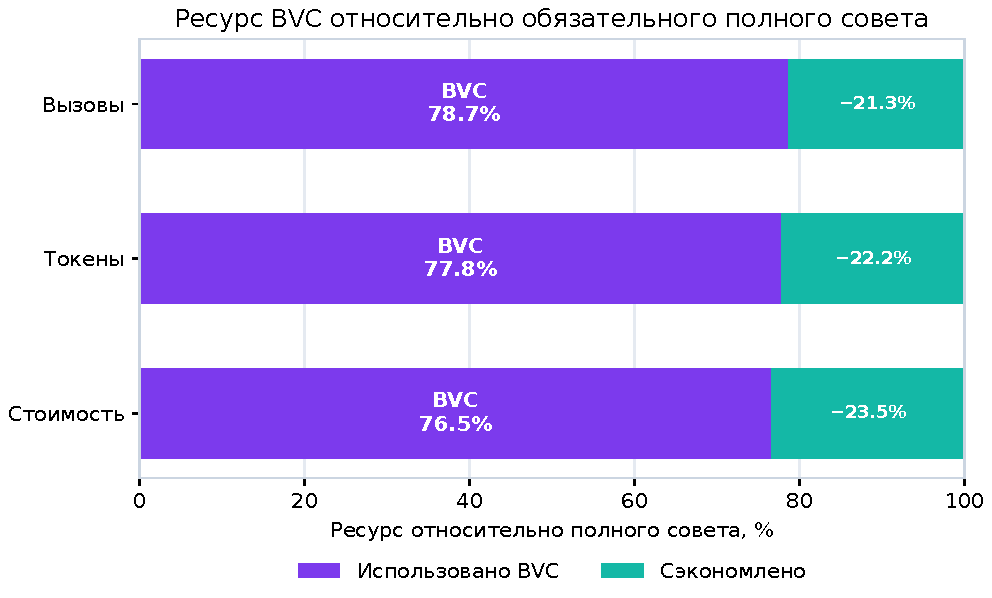
\includegraphics[width=0.9\textwidth]{fig_resource_normalized}
\caption{Нормированный расход: фиолетовая часть использована BVC, бирюзовая
часть сэкономлена относительно фиксированных 100\% полного совета.}
\label{fig:resource}
\end{figure}

В среднем на одной задаче BVC сохранил \num{\TokensSavedTask} токенов,
\num{2.13} вызова и \num{\CostSavedTask} руб. При этом экономия токенов
(22,2\%) близка к экономии вызовов (21,3\%). Это показывает, что основной
механизм результата --- именно пропуск четырёх critique-вызовов, а не
случайное сокращение длины отдельных ответов.

Фактический объём по задачам неоднороден. Медиана BVC равна 190\,866 токенов,
межквартильный диапазон --- от 180\,212 до 308\,979; у полного совета
медиана равна 307\,980, диапазон --- от 298\,149 до 318\,023. Двухмодальная
структура BVC закономерно отражает два маршрута.

\begin{figure}[H]
\centering
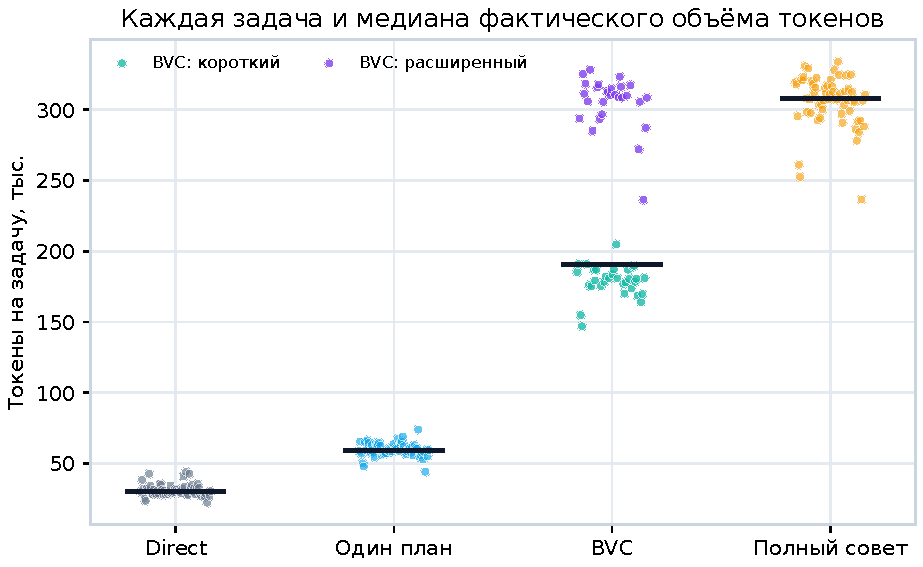
\includegraphics[width=0.9\textwidth]{fig_tokens_boxplot}
\caption{Каждая задача и медиана токенов; для BVC цвет разделяет два маршрута.}
\label{fig:token-box}
\end{figure}

\begin{table}[H]
\centering
\caption{Подгруппы BVC по фактически выбранному маршруту.}
\label{tab:route-groups}
\begin{tabular}{@{}lrrrr@{}}
\toprule
Маршрут & Задач & Вызовов & Средние токены & Средняя цена, руб.\\
\midrule
6 вызовов, без критики & \BVCShort & 192 & \num{\BVCShortTokensMean} &
\num{\BVCShortCostMean}\\
10 вызовов, с критикой & \BVCExtended & 280 &
\num{\BVCExtendedTokensMean} & \num{\BVCExtendedCostMean}\\
\bottomrule
\end{tabular}
\end{table}

Короткий маршрут в среднем стоил \num{\BVCShortCostMean} руб. на задачу,
расширенный --- \num{\BVCExtendedCostMean} руб. Разность
\(\num{16.84}\) руб. описывает разность подгрупп, но не является чистой
каузальной ценой второго раунда: состав задач и длины ответов также различаются.
Все пять успешных BVC-задач оказались
в короткой подгруппе; расширенная подгруппа содержала больше hard и very hard
задач. Эти числа описывают маршрутизацию наблюдаемой выборки и не позволяют
каузально заключить, что отказ от критики повышает качество.

\subsection{Парная экономия по задачам}

Агрегированная сумма может скрывать задачи, на которых адаптивный маршрут
оказался длиннее из-за вариации ответа. Поэтому для каждого instance вычислена
парная разность
\[
\Delta T_i=T_{i,\mathrm{fixed}}-T_{i,\mathrm{BVC}}.
\]
Положительное значение означает экономию BVC. Сумма всех \(\Delta T_i\)
равна \num{\TokensSaved} токенов. На \TokensOverrunTasks{}/60 задачах
\(\Delta T_i<0\), то есть BVC израсходовал больше токенов; максимальный
перерасход составил \num{\TokensOverrunMax} токенов. Все такие случаи относятся
к расширенному маршруту, где оба режима выполняли по 10 вызовов, а разность
создавалась длиной независимо сгенерированных ответов.

\begin{figure}[H]
\centering
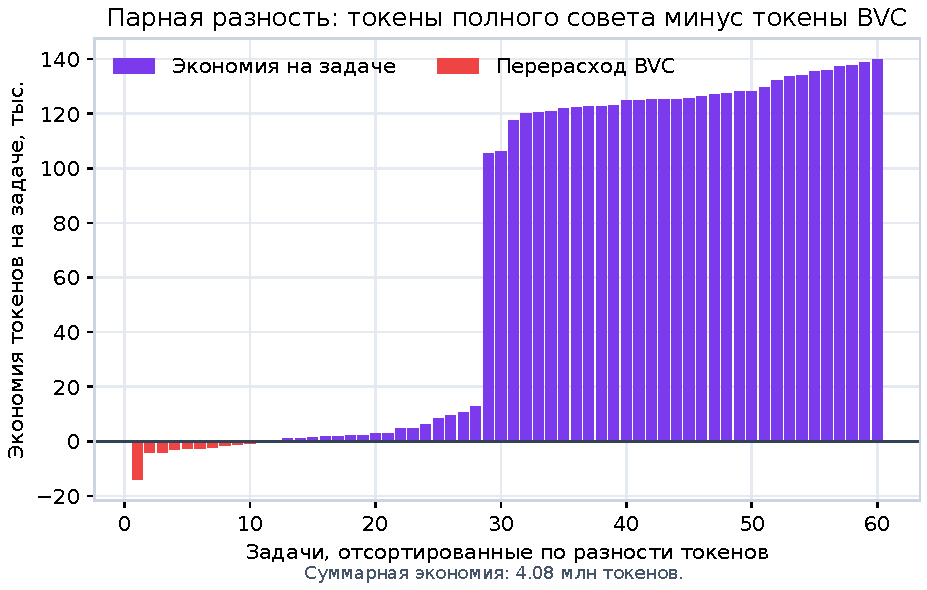
\includegraphics[width=0.92\textwidth]{fig_task_token_savings}
\caption{Распределение парной экономии токенов по 60 задачам.}
\label{fig:task-savings}
\end{figure}

Для проверки того, что агрегированная экономия не создаётся несколькими
выбросами, дополнительно рассчитаны парные разности
\(\Delta X_i=X_{i,\mathrm{fixed}}-X_{i,\mathrm{BVC}}\). Это расширенный
описательный анализ, выполненный после основной замороженной проверки:
среднее повторно оценивалось в 10\,000 bootstrap-выборках внутри тех же
трёх страт. Средняя экономия на задачу составила
\(\num{\CallsSavedTaskMean}\) вызова, \num{\TokensSavedTask} токенов и
\num{\CostSavedTask} руб. Соответствующие 95\% интервалы равны
\([\num{\CallsSavedTaskMeanLow};\num{\CallsSavedTaskMeanHigh}]\) вызова,
\([\num{\TokensSavedTaskMeanLow};\num{\TokensSavedTaskMeanHigh}]\) токенов
и \([\num{\CostSavedTaskMeanLow};\num{\CostSavedTaskMeanHigh}]\) руб.
Интервалы приведены как описание разброса на этой замороженной смеси страт.
Положительность экономии вызовов следует из конструкции gate при доле критики
меньше единицы и не является отдельной проверяемой гипотезой; для токенов и
рублей отдельные парные разности могут быть отрицательными.

\begin{figure}[H]
\centering
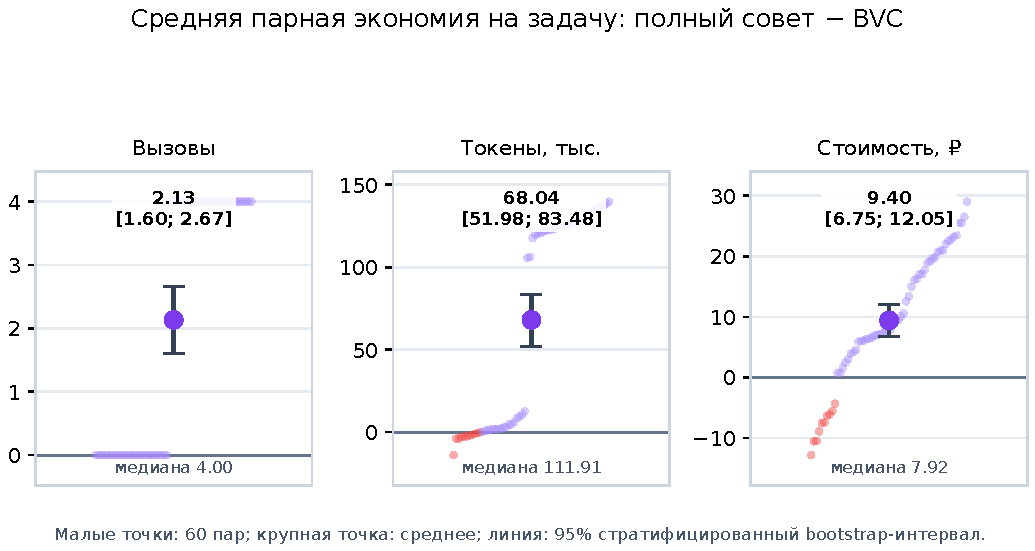
\includegraphics[width=0.92\textwidth]{fig_resource_paired_effects}
\caption{Средняя парная экономия и 95\% стратифицированные
bootstrap-интервалы; положительный знак означает меньший расход BVC.}
\label{fig:resource-paired}
\end{figure}

Медианы парной экономии равны \num{\TokensSavedTaskMedian} токенов и
\num{\CostSavedTaskMedian} руб. Эти величины не обязаны иметь один и тот же
коэффициент пересчёта: рублёвая цена является линейной комбинацией трёх
категорий токенов с разными весами, а их доли меняются между задачами. Поэтому
медиана суммы токенов не определяет медиану стоимости. Прямой пересчёт всех
60 пар даёт именно 7,92 руб.; на \CostOverrunTasks{}/60 задачах наблюдался
рублёвый перерасход, максимальный --- \num{\CostOverrunMax} руб.

\begin{figure}[H]
\centering
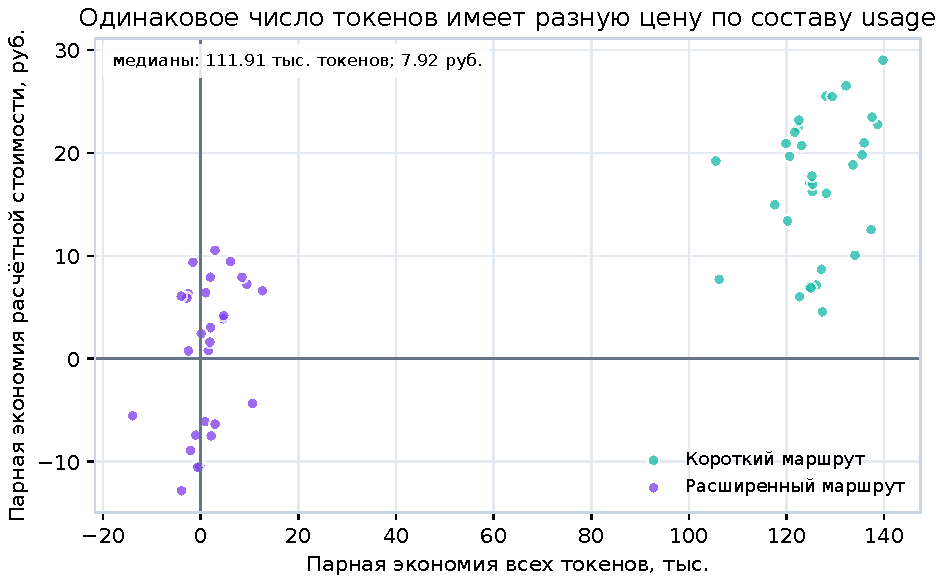
\includegraphics[width=0.92\textwidth]{fig_tokens_cost_relation}
\caption{Связь экономии всех токенов с тарифно-взвешенной экономией стоимости.}
\label{fig:tokens-cost-relation}
\end{figure}

\subsection{Из чего складывается денежная экономия}

Стоимость разложена на кэшированный вход, некэшированный вход и выход.
Поскольку каждая роль повторно получает значительную часть общего кодового
контекста, кэширование заметно снижает цену входа, но не устраняет стоимость
выходных решений и critique-ответов.

\begin{figure}[H]
\centering
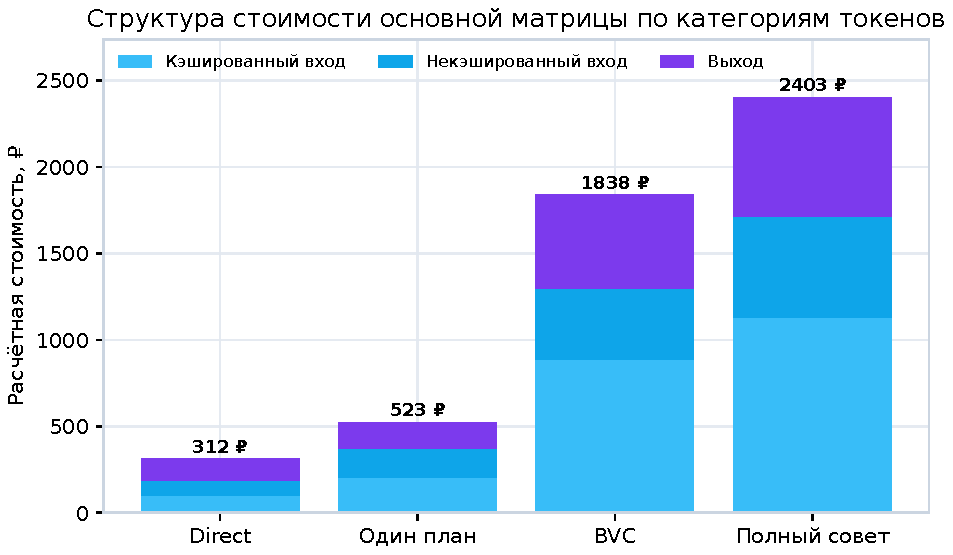
\includegraphics[width=0.9\textwidth]{fig_cost_components}
\caption{Компоненты расчётной стоимости основной серии.}
\label{fig:cost-components}
\end{figure}

\subsection{Функциональный результат как контроль экономии}

Официальный evaluator признал решёнными \BVCResolved{}/60 задач BVC и
\FixedResolved{}/60 задач полного совета. Парная таблица имеет вид:

\begin{table}[H]
\centering
\caption{Попарное пересечение функциональных исходов BVC и полного совета.}
\label{tab:paired-fixed}
\begin{tabular}{@{}lrrr@{}}
\toprule
 & Полный совет: решено & Полный совет: не решено & Всего\\
\midrule
BVC: решено & 5 & 0 & 5\\
BVC: не решено & 1 & 54 & 55\\
\midrule
Всего & 6 & 54 & 60\\
\bottomrule
\end{tabular}
\end{table}

Разложение по фактическому маршруту уточняет источник единственной
дискордантной пары:

\begin{table}[H]
\centering
\caption{Функциональные исходы BVC и полного совета по маршруту BVC.}
\label{tab:route-outcomes}
\begin{tabular}{@{}lrrr@{}}
\toprule
Маршрут BVC & Задач & BVC решено & Полный совет решено\\
\midrule
Короткий, 6 вызовов & \BVCShort & \BVCShortResolved & \FixedShortResolved\\
Расширенный, 10 вызовов & \BVCExtended & \BVCExtendedResolved & \FixedExtendedResolved\\
\bottomrule
\end{tabular}
\end{table}

Единственная задача, решённая только полным советом
(\code{django\_\_django-13128}), принадлежит расширенной подгруппе. В ней оба
режима выполнили критику и имели одинаковую структуру из 10 вызовов. Поэтому
наблюдаемую разность нельзя приписать решению gate о пропуске критики; при
недоступном provider seed два структурно одинаковых запуска всё равно могли
сгенерировать разные планы и patch.

Разность долей равна \(-1{,}7\) \pp, 95\% стратифицированный
bootstrap-интервал --- \([-5{,}0;0{,}0]\) \pp, точное
\(p_{\mathrm{McNemar}}=1{,}0\). Следовательно, данные не доказывают равенство
методов, но показывают, что пять из шести успехов полного совета сохранены
при сокращении ресурсов более чем на одну пятую.
Нулевая верхняя граница bootstrap-интервала следует из пустой клетки
«только BVC»: в каждой resampling-реплике разность BVC--полный совет
неположительна. Это свойство наблюдаемой матрицы, а не самостоятельное
свидетельство о знаке эффекта в генеральной совокупности.

Для каждой отдельной доли Wilson-интервалы широки: BVC 8,3\%
\([3{,}6;18{,}1]\), полный совет 10,0\% \([4{,}7;20{,}1]\).
График всех методов нужен для контекста, а вывод об экономии строится на
структурно наиболее близкой паре BVC--полный совет.

\begin{figure}[H]
\centering
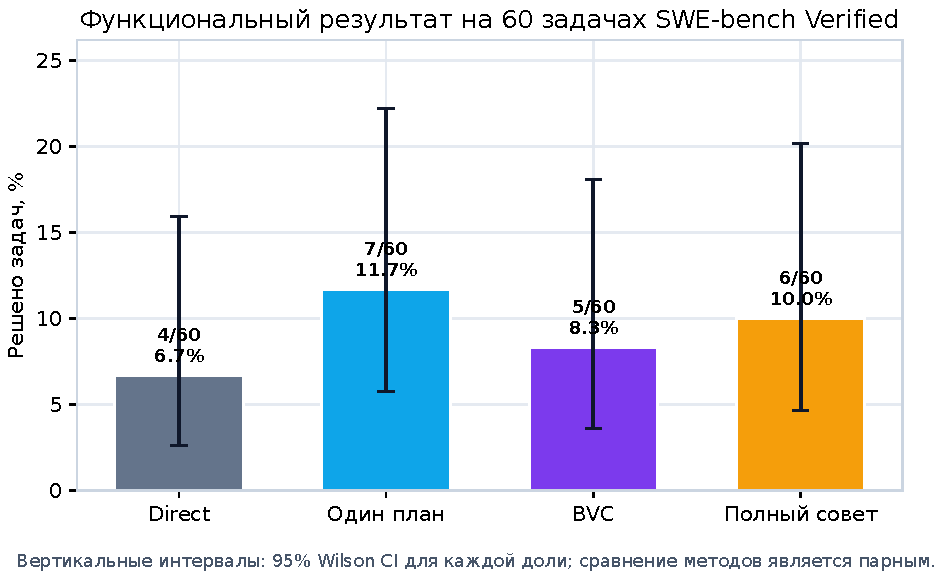
\includegraphics[width=0.9\textwidth]{fig_success_wilson}
\caption{Доли решённых задач и 95\% Wilson-интервалы.}
\label{fig:success}
\end{figure}

В общем протоколе заранее заявленным первичным сравнением было BVC против
одного плана с допустимой потерей \(-5\) \pp. Его интервал
\([-10{,}0;+3{,}3]\) пересекает этот порог: нижняя граница лежит ниже
\(-5\) \pp, поэтому неухудшаемость BVC не установлена.

\subsection{Цена одного наблюдаемого успеха и точка безубыточности}

Описательная стоимость одного решённого экземпляра задачи:
\[
R_{\mathrm{success}}=\frac{R_{\mathrm{total}}}{N_{\mathrm{resolved}}}.
\]
Для BVC она составила \num{\BVCCostResolved} руб., для полного совета ---
\num{\FixedCostResolved} руб., то есть на \CostResolvedSavedPct\% меньше.
Показатель не является независимой статистической оценкой: знаменатель мал,
а решённые задачи различаются. Чувствительность к изменению знаменателя на
одну задачу показывает хрупкость этой нормировки:

\begin{center}
\begin{tabular}{@{}lrrr@{}}
\toprule
Успехов BVC & 4 & 5 (наблюдалось) & 6\\
\midrule
Руб./успех & 459,62 & 367,69 & 306,41\\
\bottomrule
\end{tabular}
\end{center}

Наблюдаемая цена полного совета равна 400,44 руб./успех. Следовательно,
операционная нормировка BVC лучше только при пяти и более успехах; потеря
одного успеха меняет её направление. Это иллюстрация чувствительности, а не
доказательство экономического превосходства.

\section{Практическая ценность и применение}

\subsection{Что именно доказано измерениями}

Наиболее сильный вывод не требует экстраполяции качества. Gate реально
выбрал оба маршрута и тем самым:
\begin{itemize}
  \item исключил \CallsSaved{} из 600 потенциальных вызовов;
  \item сократил объём на \num{\TokensSaved} токенов;
  \item уменьшил расчётную стоимость на \num{\CostSaved} руб.;
  \item сохранил пять общих с полным советом функциональных успехов.
\end{itemize}
Это является прямой эмпирической демонстрацией адаптивной экономии. В среднем
на одну задачу алгоритм исключил 2,13 вызова, \num{68039} токенов и 9,40 руб.
расчётной стоимости. Главная польза здесь операционная: команда получает
глубокую проверку там, где gate обнаруживает основания для неё, не оплачивая
одинаковый раунд критики для каждой задачи.

\subsection{Как использовать результат в Xynapse}

Дипломная архитектура Xynapse предполагает явное включение BVC до первой
правки \cite{khalilov2026}. Эксперимент уточняет продуктовый контракт.
Интерфейс может заранее показывать диапазон 6--10 вызовов, после первого
раунда --- фактическое решение gate и его числовые основания, после
завершения --- токены и расчётную стоимость. Пользователь получает не
неограниченный \enquote{рой}, а проверяемый этап планирования с фиксированной
верхней границей.

Для мониторинга полезны четыре метрики:
\begin{enumerate}
  \item доля задач, направленных на критику;
  \item средняя и 95-й процентиль токенов на маршрут;
  \item функциональный outcome после официальных тестов;
  \item цена решённой задачи относительно полного совета.
\end{enumerate}
При смене модели, тарифа или контекстного окна те же формулы позволяют
пересчитать экономику без изменения определения алгоритма.

\section{Границы интерпретации}

Эксперимент использует 60 задач и одну конфигурацию модели; низкое число
успехов создаёт широкие интервалы качества. Наблюдаемая цена зависит от
замороженного тарифа. Расширенный маршрут получал задачи после диагностического
сигнала, поэтому подгруппы короткого и полного маршрутов не рандомизированы.
Не проверялись равнобюджетные альтернативы вроде best-of-10 direct,
self-consistency или цикла \enquote{patch--ошибка--повтор}. Поэтому работа
изолирует экономию адаптивного gate относительно собственной неадаптивной
версии, но не доказывает, что многоролевая декомпозиция является лучшим способом
потратить 6--10 вызовов. Контекст был ограничен замороженным BM25-пакетом, а
генератор не имел инструментального цикла с обратной связью тестов; абсолютные
доли успеха относятся именно к этому однопроходному контуру. Agentless и
SWE-agent показывают, что локализация, отбор patch и агентно-компьютерный
интерфейс являются самостоятельными факторами результата
\cite{xia2024agentless,yang2024sweagent}.
Кроме того, последующий аудит \dataset{} показал остаточные проблемы тестов
и возможную контаминацию; поэтому набор больше не рекомендуется как мера
текущей frontier-способности моделей \cite{openai2026verifiedlimits}. В
данной работе он используется уже не как рейтинг модели, а как один
замороженный исполняемый тест для парного сравнения четырёх методов на
одинаковых задачах. Это сохраняет смысл утверждения
\enquote{в этой матрице и при этом evaluator}, но запрещает переносить
проценты на всю разработку. По этим причинам статья утверждает адаптивную
экономию, но не статистическое неухудшение и не преимущество точности.

Три подготовленные статьи используют одну и ту же основную матрицу из 240
запусков, но отвечают на разные вопросы: настоящая работа анализирует бюджет,
сопутствующая методическая работа --- аудит контура, а третья --- заранее
включаемый пользовательский сценарий и разговорную переформулировку. Это не
три независимых эксперимента; совпадающие агрегаты между статьями должны
совпадать буквально.

\section{Заключение}

BVC превратил многоролевую проверку из режима с постоянными 10 вызовами в
ограниченный, объяснимый процесс с фактическим средним 7,87 вызова. На 60 реальных
задачах это дало экономию 21,3\% вызовов, 22,2\% токенов и 23,5\%
расчётной стоимости относительно полного совета. Функциональный контроль
зафиксировал 5 решений BVC против 6 у полного совета, причём пять успехов
совпали. Практический результат состоит в том, что предложенный в дипломе
Xynapse/BVC механизм \cite{khalilov2026} получил количественно проверенную
форму: полный inference-time бюджет можно включать по наблюдаемому
расхождению, сохраняя заранее известную верхнюю границу, прозрачный учёт
стоимости и воспроизводимое основание каждого решения. Именно это делает BVC
практически сильным алгоритмом управления проверкой: он не обещает
\enquote{магическое} улучшение, а даёт измеримый контроль над глубиной анализа.

\section*{Декларации}

Внешнее финансирование и конфликт интересов отсутствуют. LLM-системы
использовались в эксперименте как исследуемые генераторы, при подготовке
разговорных переформулировок и при редакционной проверке рукописи. Все числа и
графики повторно строятся программно из сохранённых JSON/JSONL; ответственность
за дизайн, интерпретацию и окончательный текст несёт автор. ВКР
\cite{khalilov2026} цитируется как источник архитектуры Xynapse/BVC, а не как
источник экспериментальных чисел.

\printbibliography[title={Литература}]
\end{document}
